The last prototype developed in TRITIUM experiment and the second thought to be the final versión of the Tritium detector module was Tritium-IFIC 2, which is shown in the figure \ref{fig:TritiumIFIC2}, A.

\begin{figure}[h]
\centering
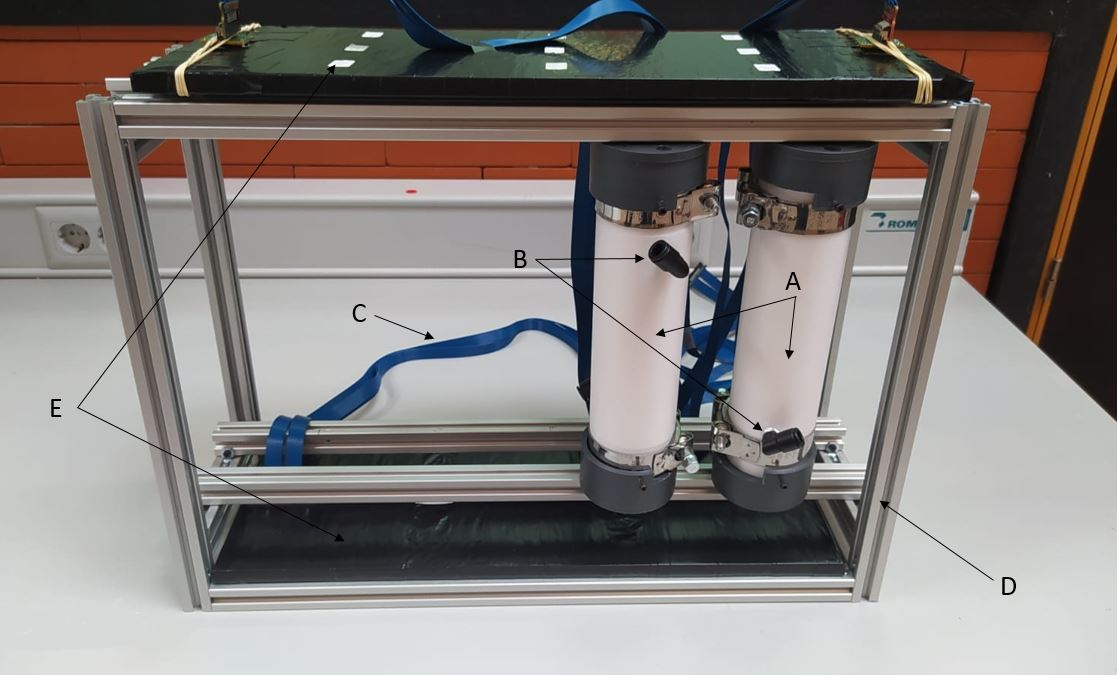
\includegraphics[scale=0.4]{5Prototypes/53FinalPrototypes/532TritiumIFIC2/Tritium_IFIC_2_full_module.jpg}
\caption{Tritium-IFIC 2 prototype.\label{fig:TritiumIFIC2}}
\end{figure}

This prototype was designed and built in the IFIC workshop and it consists of a cylindrical teflon vessel, shown in the figure \ref{fig:Tritium-IFIC2_vessels}, whose shape is similar to the one used in Tritium-Aveiro 0 prototype, whose internal length and diameter are $200~\mm$ and $36~\mm$ respectively.

\begin{figure}[h]
 \centering
  \subfloat[Tritium-IFIC 2 vessel]{
   \label{subfig:Tritium_IFIC_2_vessel}
    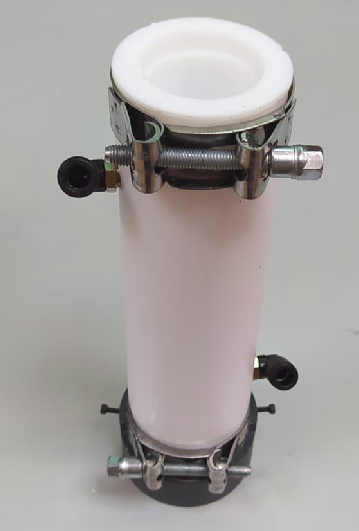
\includegraphics[angle=0, width=0.35\textwidth]{5Prototypes/53FinalPrototypes/532TritiumIFIC2/Tritium_IFIC_2_vessel1.png}}
    %\newline
  \subfloat[Tritium-IFIC 2 vessel with PVC caps]{
   \label{subfig:TritiumIFIC2_vessel_with_PVC_caps}
    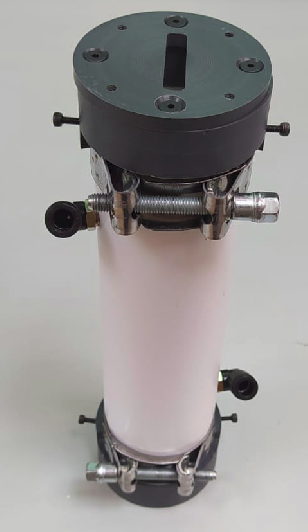
\includegraphics[angle=0, width=0.3\textwidth]{5Prototypes/53FinalPrototypes/532TritiumIFIC2/Tritium_IFIC_2_vessel2.png}}
 \caption{Tritium-IFIC 2 teflon vessel.}
 \label{fig:Tritium-IFIC2_vessels}
\end{figure}

This prototype contains $800$ no-clad scintillating fibers, model BCF-12, with a length of $200~\mm$. We can check that, as we have said, many more fibers are used than the Tritium-Aveiro 0 prototype which are arranged in less volume.

The fibers used are cut, polished and cleaned with the conditioning processes previously shown in the section \ref{subsubsec:ConditioningProcess} since, at that time, the development of the automatic polishing machine had been completed.

These fibers are freely arranged, with a density that allows water to flow through the fibers and two PMMA windows located at the ends of the fiber bundle were used to read this system, similar to the Tritium-Aveiro 0 prototype. 

The width of the PMMA optical windows used is $5~\mm$, which is sufficient to guarantee radiosecurity since we are working at very low water pressure  and two clamps are used to ensure the watertightness of the prototype, similar to the Tritium-Aveiro 0 prototype. We have checked that the transmission coefficient, shown in figure \ref{fig:PMMATransmissionSpectrum}, is not affected by the little difference of the PMMA width used in both prototypes.

As can be seen in the figure \ref{fig:TritiumIFIC2}, B, and figure \ref{fig:Tritium-IFIC2_vessels}, a water inlet/outlet was installed in the teflon vessel of this prototype to allow a constant water flux through the prototype, similar to the Tritium-Aveiro 0 prototype.

For the first laboratory measurements, two PMTs were used, model R8520-460 from the Hamamatsu Photonics company \cite{DataSheetPMTs}, which is useful to understand the results and compare them with the results obtained with the previous prototypes. However, measurements with SiPM arrays have already started whose output signal is connected to PETSYS system through flat wires as can be seen in the figure \ref{fig:TritiumIFIC2}, C.

We have to take into account that our final objective will be to install this prototype in Arrocampo dam using SiPM arrays readout by the PETSYS system. This is the reason why we have not developed a electronics chain to process and analyze the PMT signals of this prototype.

Like the Tritium-Aveiro 0 prototype, although PETSYS has a graphical user interface, shown in figure \ref{fig:GUI_PETSYS}, which allows controlling all the different options such as the voltage with which we feed the SiPM arrays, the thresholds used, etc., normally it will be controlled remotely via computer terminal. 

\begin{figure}[h]
\centering
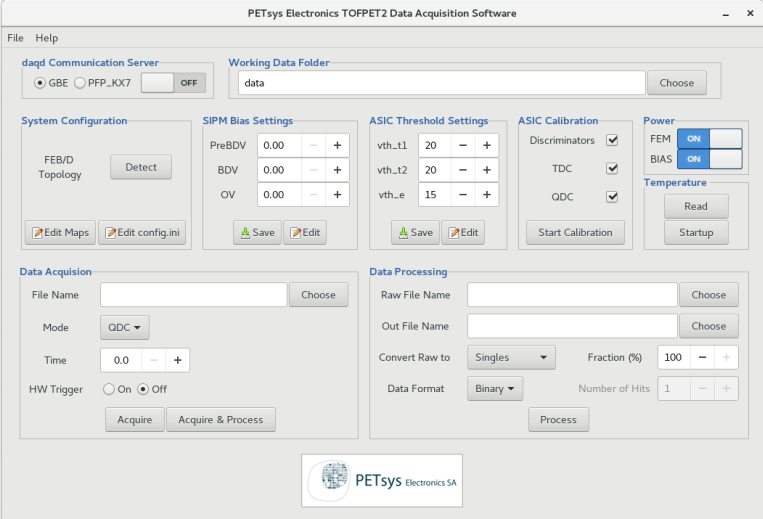
\includegraphics[scale=0.4]{5Prototypes/53FinalPrototypes/532TritiumIFIC2/GUI_PETSYS.png}
\caption{Graphical User Interface (GUI) of PETSYS.\label{fig:GUI_PETSYS}}
\end{figure}

Two PVC caps, located at both ends of the prototype, figure \ref{subfig:TritiumIFIC2_vessel_with_PVC_caps}, were used to work with the SiPMs in a light-tight envirnoment and an aluminum structure, shown in figure \ref{fig:TritiumIFIC2}, was designed and built to house up to 10 tritium-IFIC 2 modules and two cosmic vetos, shown in figure \ref{fig:TritiumIFIC2}, E.

At this point we should note that, in the available space of the lead shielding, explained in section \ref{subsec:SetUpPassiveShield}, we can accommodate up to 5 structures like the one shown in figure \ref{}. It means that our final Tritium detector is prepared to have up to 50 Tritium-IFIC 2 modules and 10 different cosmic vetos. It means that, due to the reason that our detector scales with the number of tritium modules used, the results obtained with the tritium detector can improve the results obtained with the tritium-ific 2 prototype by a factor of 50.

Two identical Tritium-IFIC 2 prototypes were built and, similar to the Tritium-IFIC 0 prototype, one of them was filled with ultrapure water and used to measure the background and the other was filled with a radioactive liquid source of tritium and used to measure the signal. The volume used in both cases was $82~\milli\liter$.

The activity of the tritium source used for this prototype is $10~\kilo\becquerel/\liter$ (uncertainty of $2.24\%$), which was prepared by diluting a sample of tritiated water explained in appendix \ref{App:TritiumSourcePreparation} with ultrapure water until the desired activity was achieved.

The results of this prototype is shown in figure section \ref{subsec:ResultsTritiumIFIC2}, where they will be compared with the results of the previous prototypes and, specially, with Tritium-Aveiro 0 prototype to choose the design with the best results.